
\subsection{Diagramas de casos de uso}
De forma a ser possível visualizar graficamente todas as ações que os 
atores conseguem realizar e para melhorar a comunicação com as 
partes interessadas do projeto, foram desenvolvidos diagramas de 
casos de uso.

\subsubsection{Casos de uso Fórum}
Na imagem representada abaixo (Figura~\ref{fig:9}) é possível 
visualizar o diagrama de casos de uso para o fórum.
Neste, o utilizador poderá ver as listagens de tópicos em destaque, tópicos mais recentes, caso seja um 
técnico poderá também ver os tópicos privados e os seus tópicos. 
O utilizador poderá também pesquisar por tópicos,  dos quais ele poderá selecionar um tópico 
específico para visualizar. 
O técnico poderá, além disso, criar um novo tópico onde se dirigirá para a criação de tópicos,
nesta o técnico será obrigado a inserir um título, descrição e tipo do tópico para o criar, 
mas também poderá inserir imagens e indicar produto referente.
Para finalizar a criação o técnico poderá confirmar ou cancelar o processo. 

\begin{figure}[htb]
    \centering
    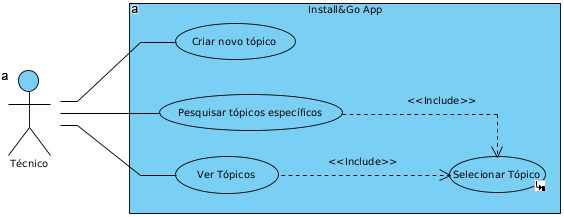
\includegraphics[width=0.6\textwidth]{images/diagramas/casos_de_uso/use_case_forum.png}
    \caption{Diagrama de casos de uso de fórum}
    \label{fig:9}
\end{figure}

\subsubsection{Casos de uso de pesquisar tópicos}

O utilizador poderá realizar a pesquisa por tópicos específicos, 
esta pesquisa poderá ser realizada por escrito onde o utilizador indica o assunto a pesquisar, esta poderá ser filtrada.
O utilizador poderá também pesquisar por tópicos específicos referentes a um produto, no qual o utilizador 
lê o código QR do produto, sendo este pesquisado no servidor Motorline, e de seguida poderá realizar 
uma pesquisa por escrito, sendo listado apenas tópicos com o produto em questão referenciado.

\begin{figure}[htb]
    \centering
    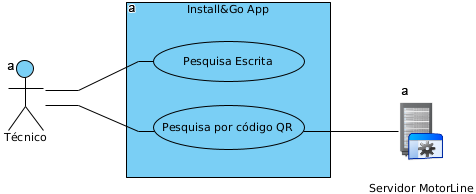
\includegraphics[width=0.6\textwidth]{images/diagramas/casos_de_uso/use_case_forum_search.png}
    \caption{Diagrama de casos de uso de pesquisa de tópicos}
    \label{fig:10}
\end{figure}

\subsubsection{Casos de uso ver detalhes de tópico}

Assim que um utilizador seleciona um tópico é direcionado para os 
detalhes de tópico, onde apenas consegue visualizar o tópico e os comentários do mesmo.

Já o técnico consegue também responder ao tópico e, caso seja do mesmo, este consegue finalizar 
o tópico, selecionar a melhor resposta e remover, eliminar e alterar a visibilidade do tópico.

\begin{figure}[htb]
    \centering
    
    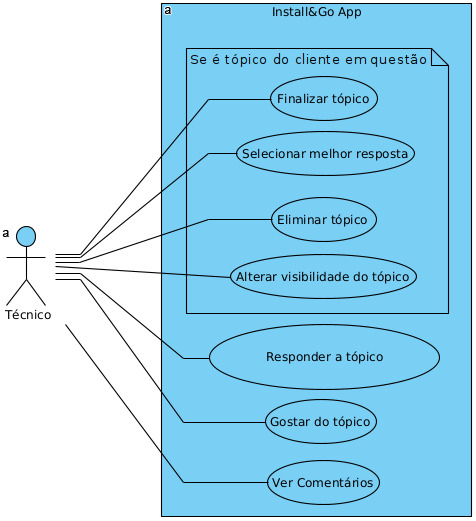
\includegraphics[width=0.5\textwidth]{images/diagramas/casos_de_uso/use_case_topic_details.png}
    \caption{Diagrama de casos de uso de detalhes de tópico}
    \label{fig:11}
\end{figure}

\subsubsection{Casos de uso ver comentários}

O técnico quando decide visualizar os comentários consegue responder a 
um comentário e gostar de uma resposta ou comentário, caso este 
seja seu ainda o consegue apagar.

\begin{figure}[htb]
    \centering
    
    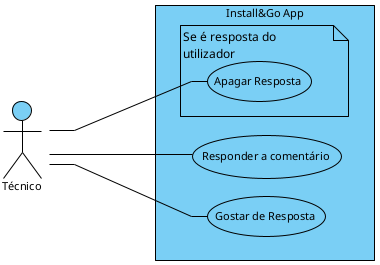
\includegraphics[width=0.5\textwidth]{images/diagramas/casos_de_uso/use_case_topic_comments.png}
    \caption{Diagrama de casos de uso de ver comentários}
    \label{fig:12}
\end{figure}

\subsubsection{Casos de uso ativação de conta}

Assim que uma conta é confirmada, um email de ativação é enviado para técnico e esta deverá ser ativada,
para isto o código deverá ser indicado pelo técnico para se proceder à ativação da conta. Este poderá,
em caso de necessidade, pedir o reenvio do código de ativação, o qual será gerado novamente e reenviado.

\begin{figure}[htb]
    \centering
    
    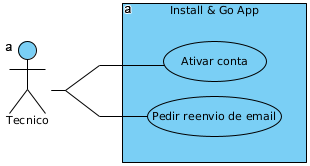
\includegraphics[width=0.5\textwidth]{images/diagramas/casos_de_uso/use_case_account_validation.png}
    \caption{Diagrama de casos de uso de ativação de conta}
    \label{fig:13}
\end{figure}

\subsubsection{Casos de uso perfil}

Sempre que o técnico desejar alterar alguma informação sua, poderá alterar o seu nome, email e imagem 
de perfil.

\begin{figure}[htb]
    \centering
    
    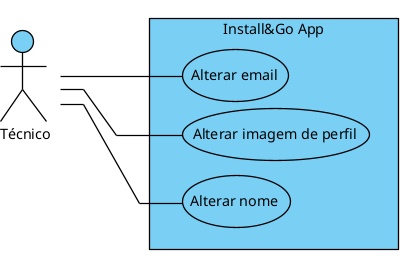
\includegraphics[width=0.5\textwidth]{images/diagramas/casos_de_uso/use_case_perfil.png}
    \caption{Diagrama de casos de uso de ativação de conta}
    \label{fig:14}
\end{figure}

\newpage

\subsubsection{Casos de uso notificações}

Sempre que o técnico desejar ver as suas notificações, este poderá selecionar as suas notificações, este
terá também a possibilidade de alterar a configuração das suas notificações, para apenas as receber 
por email ou push ou então ambas e poderá também personalizar cada método para receber
relatório diário de notificações ou então notificações em tempo real.

\begin{figure}[htb]
    \centering
    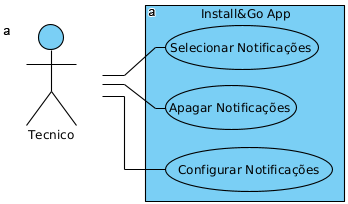
\includegraphics[width=0.5\textwidth]{images/diagramas/casos_de_uso/use_case_notificacoes.png}
    \caption{Diagrama de casos de uso de ativação de conta}
    \label{fig:15}
\end{figure}

\subsubsection{Casos de uso gestão de recursos humanos}

Uma empresa poderá registar contas para os seus técnicos em seu nome, indicando o seu email e nºcontribuinte,
esta poderá também impedir acesso a estas contas ou remover completamente a conta da aplicação.

\begin{figure}[htb]
    \centering
    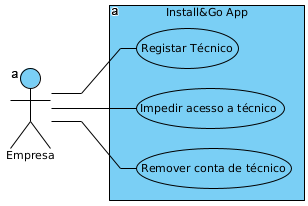
\includegraphics[width=0.5\textwidth]{images/diagramas/casos_de_uso/use_case_rec_humanos.png}
    \caption{Diagrama de casos de uso de ativação de conta}
    \label{fig:16}
\end{figure}